\begin{slide}
\heading{Tuning}

We want to tune the program to run quickly.  There are two questions to
consider: 
%
\begin{itemize}
\item How many workers should we use?

\item Should we use buffered channels?
\end{itemize}
%
We can run some experiments to try to obtain (at least) partial answers to
these; although the answers are likely to vary with the architecture.

We consider $n$ (the number of intervals) as an input: under different
circumstances, we might want to use different values for~$n$.

%% Each experiment was as follows:
%% %
%% \begin{itemize}
%% \item The experiments were run on a 32-core server (two 2.1GHz Intel(R)
%% Xeon(R) E5-2683 CPUs with hyperthreading enabled).

%% \item 
%% Each instance estimated $\int_{-100000}^{+100000} x^2 \cos x \, \mbox{d}x$.
%% \end{itemize}

\end{slide}

%%%%%

\begin{slide}
\heading{How many workers to use?}

The experiments to decide the number of workers were as follows.
%
\begin{itemize}
\item The experiments were run on a 32-core server (two 2.1GHz Intel(R)
Xeon(R) E5-2683 CPUs with hyperthreading enabled).

\item 
Each instance calculated an approximation of $\int_{-100000}^{+100000} x^2
\cos x \, \mbox{d}x$.

\item
Various different sizes of $n$ were used between $2^{16}$ and $2^{28}$; each
observation calculated the integral $2^{28}/n$ times (so all observations were
about the same amount of work).

\item
Each instance used buffered channels with capacity 16.

\item
For each choice of $n$, various values of |nWorkers| were used.

\item
For each choice of parameters, multiple observations were made, and the mean
and 95\% confidence interval calculated.
\end{itemize}
\end{slide}

%%%%%

\begin{slide}
\label{slide:not-bag-of-tasks}
% scala -cp .:/home/gavinl/Scala/SCL:/home/gavinl/Scala/Util
% TrapeziumExperiment  --buffering 16 --doLog --strict --server on casteret
\begin{tikzpicture}
\begin{semilogxaxis}[
%  title = Timing experiment on the numerical integration example,
  ylabel = Time (ms),
  legend pos = north west,
  height = 0.98\textheight,
  width = 0.98\textwidth,
  scaled ticks = false,
  xlabel = Number of workers,
  xmin = 1,
  ymin = 0,
  ymax = 12000,
  log basis x=2
]

\addplot+[error bars/.cd, y dir=both,y explicit] coordinates {
  (512,66906.464174) +- (0,92.47266334851669)
  (256,33389.1291968) +- (0,90.82336557462699)
  (128,15921.3202264) +- (0,49.98543102984851)
  (64,7039.0096576000005) +- (0,50.23851632801305)
  (32,3477.035578181818) +- (0,31.78185210316302)
  (16,2806.8691438) +- (0,24.312484048502558)
  (8,2615.551757) +- (0,18.93106961242095)
  (4,3302.8918018000004) +- (0,21.88235727705309)
  (2,4821.4516514) +- (0,46.02325040305744)
  (1,8514.2120288) +- (0,30.33328457227989)
};
\addlegendentry{$n = 2^{18}$}
\addplot+[error bars/.cd, y dir=both,y explicit] coordinates {
  (512,17062.1814972) +- (0,68.81735222663036)
  (256,8716.506757) +- (0,73.74487896789209)
  (128,4338.5419785) +- (0,38.49607339998644)
  (64,2222.2029872) +- (0,21.052171978571973)
  (32,1620.89841275) +- (0,15.931547998759857)
  (16,1630.0650955714286) +- (0,15.321734270700714)
  (8,1902.2857148666665) +- (0,18.62486316909343)
  (4,2650.8328705999998) +- (0,19.107720313879742)
  (2,4337.412955571428) +- (0,36.724920562987535)
  (1,8001.85438) +- (0,73.38146511824169)
};
\addlegendentry{$n = 2^{20}$}
\addplot+[error bars/.cd, y dir=both,y explicit] coordinates {
  (512,1799.56714182) +- (0,32.71738180547917)
  (256,1363.52716338) +- (0,39.90186193386462)
  (128,1095.88527242) +- (0,33.988211371512506)
  (64,1038.1909207200001) +- (0,28.514381918295427)
  (32,1165.1984182) +- (0,16.087338188183626)
  (16,1249.4601490975608) +- (0,12.464870189761749)
  (8,1547.3894196666668) +- (0,15.351279424345195)
  (4,2433.725179540541) +- (0,24.262446412878784)
  (2,4060.8616351428573) +- (0,37.160363653690204)
  (1,7721.093534600001) +- (0,16.821275428807958)
};
\addlegendentry{$n = 2^{24}$}
\addplot+[error bars/.cd, y dir=both,y explicit] coordinates {
  (512,750.88449698) +- (0,54.81655513026725)
  (256,727.05934538) +- (0,56.4422401788819)
  (128,567.22785174) +- (0,24.78672447780806)
  (64,635.40388552) +- (0,7.342797598787894)
  (32,869.5884367346939) +- (0,8.678497290894436)
  (16,1047.3327939666667) +- (0,10.130131408714377)
  (8,1415.1987063333333) +- (0,10.95248597983864)
  (4,2292.3979252) +- (0,22.12424125790701)
  (2,4020.0490038125) +- (0,39.83178459400462)
  (1,7704.456190600001) +- (0,46.48908448403518)
};
\addlegendentry{$n = 2^{28}$}

\end{semilogxaxis}
\end{tikzpicture}
\end{slide}

%%%%%

\begin{slide}
\heading{Discussion of results}


\begin{itemize}
\item The amount of computation each worker performs is $O(1/\sm{nWorkers})$.
  But the amount of communication grows as $O(\sm{nWorkers})$.  

\item Each of the plots initially falls roughly proportional to
$1/\sm{nWorkers}$, which is proportional to $\sm{taskSize}$, i.e.~the
per-thread computation time.  

\item For larger values of |nWorkers|, the graphs seem to grow roughly
  proportional to |nWorkers|: the communication costs dominate.

%% The plots don't fall quite this quickly because
%% the communication and thread initialisation overheads grow proportional to
%% |nWorkers|.
\end{itemize}
\end{slide}

%%%%%


\begin{slide}
\heading{Discussion of results}

\begin{itemize}
\item
For small values of $n$ (up to about $2^{20}$), the optimal number of workers
is \emph{less} than the number of machine threads.  

Informal profiling with $n = 2^{18}$ and 64 workers shows that each worker
spends less than 25\% of its time calculating the integral: most of its
time is spent waiting for a task or waiting to send its result back to the
controller.
% scala -cp .:/home/gavinl/Scala/SCL:/home/gavinl/Scala/Util TrapeziumRun -p  64 --profile --reps 100 --size 262144 --buffering 16


The extra computation is dwarfed by the communication overheads. 

%% Extra threads reduce the per-thread computation time; but this is out-weighed
%% by the thread-creation and communication overheads.  In addition, the
%% controller acts as a bottleneck.

%% Beyond the optimal point, performance falls off rapidly: the thread-creation
%% and communication overheads dominate, and these are proportional to the number
%% of threads. 

\item
For larger values of $n$, the optimal number of workers is \emph{more} than
the number of machine threads (although the graphs are quite flat in this
range).  

Having more program threads than machine threads seems to give the
scheduler more chance for load balancing (rather like the pattern we will
look at in the next chapter). 
\end{itemize}
\end{slide}

%%%%%

\begin{slide}
\heading{Experiment concerning buffering}

We can carry out a similar experiment concerning the amount of buffering.
Some details:
%
\begin{itemize}
\item Various different sizes of $n$;

\item 64 worker threads;

\item Different amounts of buffering, including 0 (i.e.~a synchronous
  channel);

\item Other details as for the previous experiment.
\end{itemize}
\end{slide}

%%%%%


\begin{slide}
\begin{tikzpicture}
\begin{axis}[
%  title = Timing experiment on the numerical integration example,
  ylabel = Time (ms),
  legend pos = north east,
  height = 0.98\textheight,
  width = 0.98\textwidth,
  scaled ticks = false,
  %title = Experiment on the benefits of buffering,
  xlabel = Amount of buffering,
  xtick = data,
  ymax = 11500,
  symbolic x coords={0,1,2,4,8,16,32}
]

\addplot+[error bars/.cd, y dir=both,y explicit] coordinates {
  (0,8462.2592822) +- (0,71.8291716679859)
  (1,8717.5518986) +- (0,32.28246028517993)
  (2,7689.2159128) +- (0,31.958312511547966)
  (4,7290.773049) +- (0,28.02600837313684)
  (8,7121.698379) +- (0,70.10106910486228)
  (16,7048.133494) +- (0,37.00548631123019)
  (32,6916.198846125) +- (0,64.53008461366746)
};
\addlegendentry{$n = 2^{18}$}
\addplot+[error bars/.cd, y dir=both,y explicit] coordinates {
  (0,4388.0311806) +- (0,27.475385173157168)
  (1,4513.1778408) +- (0,34.95224329689597)
  (2,4018.3056444) +- (0,22.21917457523661)
  (4,3841.9693617142857) +- (0,37.030434873587765)
  (8,3768.1721822222225) +- (0,33.526125808993356)
  (16,3727.4166588000003) +- (0,32.77761738824269)
  (32,3702.6007) +- (0,37.01246780279705)
};
\addlegendentry{$n = 2^{19}$}
\addplot+[error bars/.cd, y dir=both,y explicit] coordinates {
  (0,2404.4758175) +- (0,22.94106417902077)
  (1,2461.1475072) +- (0,19.04718780190071)
  (2,2276.848227) +- (0,22.250667405164858)
  (4,2216.0773136) +- (0,22.09684430334622)
  (8,2189.798469625) +- (0,20.47038679802501)
  (16,2206.429703) +- (0,15.65965855716555)
  (32,2266.3921270833334) +- (0,21.966347711391997)
};
\addlegendentry{$n = 2^{20}$}
\addplot+[error bars/.cd, y dir=both,y explicit] coordinates {
  (0,1059.8903366) +- (0,28.944775149177275)
  (1,1057.9314238) +- (0,27.07197317361198)
  (2,1043.571615) +- (0,24.609794293852193)
  (4,1029.2399809199999) +- (0,29.75125397171397)
  (8,1032.20156518) +- (0,25.80973578121811)
  (16,1043.7603336) +- (0,24.16949383797133)
  (32,1041.58398964) +- (0,25.55474698045765)
};
\addlegendentry{$n = 2^{24}$}

\end{axis}
\end{tikzpicture}
\end{slide}

%%%%%

\begin{slide}
\heading{Discussion of results}

Buffering helps for examples with more workers than the optimal number (for
the given~$n$).  Curiously, buffering of size~1 makes things slower, however.

For examples with a more appropriate number of workers (for the given~$n$),
buffering makes very little difference, in this case.  However, it might make
more difference in other examples, particularly where the time to produce and/or
process a task is more variable.
\end{slide}

% \begin{slide}
% \heading{Experimental results}

% The following table shows the time taken (in ms) to run the system, with
% \SCALA{n=63000}, on an 8 processor machine, with Just In Time compilation
% turned \emph{off} (averaged over 200 runs).
% %
% \begin{trivlist}\item[]\def\tabcolsep{1.7mm}
% \begin{tabular}{*{19}{c}}
% nWorkers: & 1 & 2 & 3 & 4 & 5 & 6 & 7 & 8 & 9 & 10 & 12 & 15 & 20\\
% time: & 165 & 108 & 85 & 70 & 60 & 55 & 52 & 51 & 59 & 59 & 55 & 52 & 51\\[2mm]
% \end{tabular}
% \end{trivlist}

% How can we explain the figures?
% \end{slide}

% %%%%%

% \begin{selfnote}
% The fastest is when each worker is on a separate processor.  (In this case the
% controller doesn't do much work.  In an example where the controller does a
% lot of work, the fastest might be when the $\# workers = \# processors - 1$.) 

% In an ideal world, it would be $1/nWorkers$ for $nWorkers \le 8$.  But there's an
% overhead, both per extra process and overall.

% Once $nWorkers > 8$, the processes have to compete for the processors, and the
% extra time for the context switches makes it slower overall.

% I don't really understand why it gets faster again for 15 and 20.
% \end{selfnote}

%% n = 630000, 100 times each, JIT off

%% nWorkers = 1      Time taken: 156.061
%% nWorkers = 2      Time taken: 109.354
%% nWorkers = 3      Time taken: 87.591
%% nWorkers = 4      Time taken: 70.119
%% nWorkers = 5      Time taken: 60.185
%% nWorkers = 6      Time taken: 55.064
%% nWorkers = 7      Time taken: 52.063
%% nWorkers = 8      Time taken: 51.971
%% nWorkers = 9      Time taken: 56.148
%% nWorkers = 10     Time taken: 58.047
%% nWorkers = 12     Time taken: 59.018
%% nWorkers = 15     Time taken: 56.04
%% nWorkers = 20     Time taken: 57.163

%%%%%

% \begin{slide}
% \heading{Experimental results}

% The following table shows the time taken (in ms) to run the system, with
% \SCALA{n=1260000} (20 times more than the previous experiment), on the same
% machine, with Just In Time compilation turned \emph{on} (again averaged over
% 200 runs).
% %
% \begin{trivlist}\item[]\def\tabcolsep{1.5mm}%
% \begin{tabular}{*{19}{c}}
% nWorkers: & 1 & 2 & 3 & 4 & 5 & 6 & 7 & 8  & 9 & 10 & 12 & 15 & 20 \\
% time:  & 152 & 157 & 134 & 117 &  100 & 80 & 74 & 69 & 63 & 64 & 64 & 65 & 67
% % time:   & 76 & 79 & 64 & 56 & 48 & 43 & 39 & 37 & 37 & 36 & 37 & 37 & 39
% \end{tabular}
% \end{trivlist}
% %
% The Just In Time compilation has an odd effect!
% \end{slide}

% %%%%%

% \begin{slide}
% \heading{Comments}

% In this case, we could have constructed the workers with the
% appropriate values for \SCALA{f, l, r, taskSize, delta}, rather than having the
% controller distribute them.  However, we wanted to illustrate the
% pattern of having a controller distribute work to the workers.
% \end{slide}

%%%%%
